\section{Überblick}

\begin{frame}
  {Flexion | Nomina}
  \onslide<+->
  \begin{itemize}[<+->]
    \item Funktion in der Nominalflexion
    \item Flexion(sklassen) der Substantive
    \item Flexion der Pronomina und Artikel
  \end{itemize}
\end{frame}

\begin{frame}
  {Flexion im Lehramtsstudium}
  \pause
  \begin{itemize}[<+->]
    \item \alert{Wir beherrschen doch alle Formen!}
      \Halbzeile
    \item Funktion der Flexionskategorien
      \begin{itemize}
        \item semantisch\slash pragmatisch
        \item \alert{systemintern} als Hilfe zu \alert{Rekonstruktion der Satzstruktur}
      \end{itemize}
      \Halbzeile
    \item Flexion im Deutschen ein ideales und gut durchschaubares Beispiel\\
      für die klassische \alert{reduktionistische} Methode der Linguistik\\
      (= Analyse der Sprache als \alert{System})
      \Halbzeile
    \item \alert{Können} vs.\ \rot{Erklären}
    \item Reaktion auf Erwerbsschwierigkeiten (L1)
    \item inkl.\ Schwierigkeiten wegen nicht-deutscher Erstsprache (L2)
  \end{itemize}
\end{frame}


\section{Funktion}

\begin{frame}
  {Was heißt Funktion?}
  \pause
  Rückgriff auf Kapitel 3:
  \pause
  \Halbzeile
  \begin{itemize}[<+->]
    \item \alert{externe} Funktion | kommunikativ, pragmatisch, textuell, kulturell, \dots
    \item \alert{interne} Funktion | innerhalb der Grammatik Relationen kennzeichnend,
      Rekonstruktion der Struktur ermöglichend, Schnittstelle zur Semantik | \rot{Kompositionalität}
    \item nicht immer trennbar
      \Halbzeile
    \item Paradebeispiel für interne Funktion | \alert{Kasussystem}
  \end{itemize}
\end{frame}

\begin{frame}
  {Numerus}
  \pause
  \begin{exe}
    \ex
    \begin{xlist}
      \ex[ ]{Die Trainerin beobachtet [einen guten Wettkampf].}
      \pause
      \ex[*]{Die Trainerin beobachtet [einen guten \rot{Wettkämpfe}].}
    \end{xlist}
    \pause
    \ex
    \begin{xlist}
      \ex[ ]{Die Trainerin beobachtet [einige gute Wettkämpfe].}
      \pause
      \ex[*]{Die Trainerin beobachtet [einige gute \rot{Wettkampf}].}
    \end{xlist}
  \end{exe}
  \pause
  \Halbzeile
  \begin{itemize}[<+->]
    \item \alert{Anzahl von Objekten ("`Gegenständen"')} | konzeptuell beim Subst motiviert
    \item notwendigerweise volatiles Merkmal beim Subst
    \item Pluraliatantum wie \textit{Ferien} oder Singulariatantum wie \textit{Gesundheit}
  \end{itemize}
\end{frame}

\begin{frame}
  {Kasus}
  \pause
  Was ist Kasus? Haben die Kasus an sich eine Bedeutung?
  \Halbzeile
  \pause
  \begin{exe}
    \ex
    \begin{xlist}
      \ex{Wir sehen \rot{den Rasen}.}
      \pause
      \ex{Wir begehen \rot{den Rasen}.}
      \pause
      \ex{Wir säen \rot{den Rasen}.}
      \pause
      \ex{Wir fürchten \rot{uns}.}
    \end{xlist}
    \pause
    \ex
    \begin{xlist}
      \ex \rot{Nächsten März} fahre ich zum Bergwandern in die Tatra.
      \ex Es waren \rot{den ganzen Tag} Menschen zum Gipfel unterwegs.
    \end{xlist}
    \pause
    \ex
    \begin{xlist}
      \ex{Sarah backt \rot{ihrer Freundin} einen Marmorkuchen.}
      \pause
      \ex{Wir kaufen \rot{dir} ein Kilo Rohrzucker.}
      \pause
      \ex{Die Mannschaft spielt \rot{mir} zu drucklos.}
      \pause
      \ex{Der Marmorkuchen schmeckt \rot{den Freundinnen} gut.}
    \end{xlist}
  \end{exe}
\end{frame}


\begin{frame}
  {Kasus | Eigenschaften}
  \pause
  \centering

  \Large
  Kasus stellt \alert{Relationen zwischen\\
  den kasustragenden Nomina und anderen Wörtern}\\
  (Verben, Präpositionen, anderen Nomina) her.\\
\end{frame}

\begin{frame}
  {Person | Deixis}
  \pause
  Was ist die grammatische Person?

  \Halbzeile
  \pause
  \begin{exe}
    \ex
    \begin{xlist}
      \ex{\alert{Ich} unterstütze den FCR Duisburg.}
      \pause
      \ex{\alert{Ihr} unterstützt den FCR Duisburg.}
      \pause
      \ex{\alert{Sie/Diese/Jene/Eine/Man\ldots} unterstützt den FCR Duisburg.}
      \pause
      \ex{\alert{Sie/Diese/Jene/Einige/\ldots} unterstützen den FCR Duisburg.}
    \end{xlist}
  \end{exe}
  \pause
  \Halbzeile
  \begin{itemize}[<+->]
    \item prototypisch beim \alert{Pronomen} funktional motiviert
    \item Substantive | statisch dritte Person
      \Halbzeile
    \item hier | \rot{deiktische Pronomina}
      \begin{itemize}[<+->]
        \item in einer Situation verweisend
        \item nur relativ zu einer Situation interpretierbar
      \end{itemize} 
  \end{itemize}
\end{frame}

\begin{frame}
  {Person | Anaphorik}
  \pause
  \begin{exe}
    \ex \alert{Sarah$_{\textnormal{1}}$} backt \rot{[ihrer Freundin]$_{\textnormal{2}}$} \gruen{[einen Kuchen]$_{\textnormal{3}}$}.\\
      \alert{Sie$_{\textnormal{1}}$} verwendet nur fair gehandelten unraffinierten Rohrzucker.
    \pause
      \ex \alert{Sarah$_{\textnormal{1}}$} backt \rot{[ihrer Freundin]$_{\textnormal{2}}$} \gruen{[einen Kuchen]$_{\textnormal{3}}$}.\\
      \gruen{Er$_{\textnormal{3}}$} besteht nur aus fair gehandelten Zutaten.
    \pause
      \ex \alert{Sarah$_{\textnormal{1}}$} backt \rot{[ihrer Freundin]$_{\textnormal{2}}$} \gruen{[einen Kuchen]$_{\textnormal{3}}$}.\\
      \rot{Sie$_{\textnormal{2}}$} soll \gruen{ihn$_{\textnormal{3}}$} zum Geburtstag geschenkt bekommen.
  \end{exe}
  \Halbzeile
  \pause
  \begin{itemize}[<+->]
    \item anaphorische Pronomina
    \item Rückverweis im Text, Satz, Diskurs
    \item gleiche Indizes zeigen Bedeutungsidentität (Korreferenz)
    \item \rot{die Indizes setzen wir, um eine bestimmte Interpretation zu markieren.}\\
      Diese Interpretation kann möglich oder unmöglich sein.
  \end{itemize}
\end{frame}

\begin{frame}
  {Genus, Geschlecht, Gender?}
  \pause
  \begin{exe}
    \ex \label{ex:genus039}
    \begin{xlist}
      \ex \alert{Die Petunie} ist \orongsch{eine Blume}.
      \ex \rot{Der Enzian} ist \orongsch{eine Blume}.
      \ex \gruen{Das Veilchen} ist \orongsch{eine Blume}.
    \end{xlist}
  \end{exe}
  \pause
  \Halbzeile
  \begin{itemize}[<+->]
    \item reine Subklassenbildung beim Substantiv
    \item nicht in Geschlecht oder Gender motiviert
    \item teilweise Korrespondenz von maskulin und männlich\\
      sowie feminin und weiblich bei Menschen bzw.\ Lebewesen
    \item \rot{aber}
      \begin{itemize}[<+->]
        \item der Mensch
        \item die Person
        \item das (menschliche) Wesen
        \item das Individuum
      \end{itemize}
  \end{itemize}
\end{frame}

\section{Nominalflexion}

\subsection{Substantive}

\begin{frame}
  {Substantive | Kasus und Numerus}
  Das traditionelle Chaos der Flexionstypen mit Kasus-Numerus-Formen\ldots\\
  \Zeile
  \pause
  \Zeile
  \resizebox{\textwidth}{!}{
    \begin{tabular}{llp{0mm}lp{2mm}llp{1mm}lp{2mm}llp{2mm}l}
      \toprule
      \multicolumn{2}{c}{} && \multicolumn{1}{l}{\textbf{Maskulinum}} && \multicolumn{4}{l}{\textbf{Maskulinum und Neutrum}} && \multicolumn{2}{l}{\textbf{Femininum}} && \multicolumn{1}{l}{\textbf{s-Flexion}} \\
      \multicolumn{2}{c}{} && \multicolumn{1}{l}{\textbf{schwach (S1)}} && \multicolumn{2}{l}{\textbf{stark (S2)}} && \multicolumn{1}{l}{\textbf{gemischt (S3)}} && \multicolumn{2}{l}{\textbf{(S4)}} && \multicolumn{1}{l}{\textbf{(S5)}} \\
      \midrule
      \multirow{4}{*}{\textbf{Sg}} & \textbf{Nom} && Mensch && Stuhl & Haus && Staat && Frau & \multicolumn{1}{l}{Sau} && Auto \\
      & \textbf{Akk} && Mensch-en && Stuhl & Haus && Staat && Frau & \multicolumn{1}{l}{Sau} && Auto \\
      & \textbf{Dat} && Mensch-en && Stuhl & Haus && Staat && Frau & \multicolumn{1}{l}{Sau} && Auto \\
      & \textbf{Gen} && Mensch-en && Stuhl-es & Haus-es && Staat-(e)s && Frau & \multicolumn{1}{l}{Sau} && Auto-s \\
      \midrule
      \multirow{4}{*}{\textbf{Pl}} & \textbf{Nom} && Mensch-en && Stühl-e & Häus-er && Staat-en && Frau-en & \multicolumn{1}{l}{Säu-e} && Auto-s \\
      & \textbf{Akk} && Mensch-en && Stühl-e & Häus-er && Staat-en && Frau-en & \multicolumn{1}{l}{Säu-e} && Auto-s \\
      & \textbf{Dat} && Mensch-en && Stühl-en & Häus-ern && Staat-en && Frau-en & \multicolumn{1}{l}{Säu-en} && Auto-s \\
      & \textbf{Gen} && Mensch-en && Stühl-e & Häus-er && Staat-en && Frau-en & \multicolumn{1}{l}{Säu-e} && Auto-s \\
      \bottomrule
    \end{tabular}
  }
\end{frame}

\begin{frame}
  {Das traditionelle Chaos als "`System"'}
  \pause
  Das geht irgendwie nach Genus und Pluralbildung, aber nicht nur\ldots\\
  \pause
  \Zeile
  \begin{center}
    \resizebox{0.8\textwidth}{!}{
    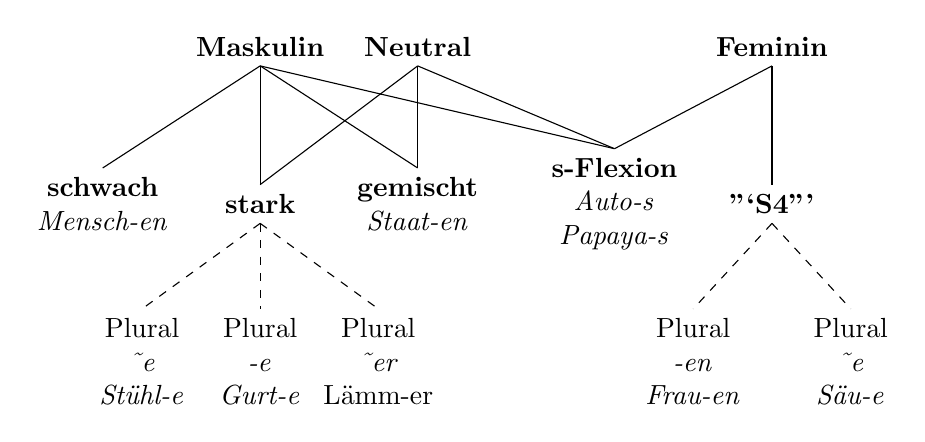
\begin{tikzpicture}[every text node part/.style={align=center}]
      \node (MaskN)    at (2,4)   {\textbf{Maskulin}};
      \node (NeutN)    at (4,4)   {\textbf{Neutral}};
      \node (FemN)     at (8.5,4) {\textbf{Feminin}};

      \node (schwachN) at (0,2)   {\textbf{schwach}\\\textit{Mensch-en}};
      \node (starkN)   at (2,2)   {\textbf{stark}};
      \node (gemistN)  at (4,2)   {\textbf{gemischt}\\\textit{Staat-en}};
      \node (sFlexN)   at (6.5,2) {\textbf{s-Flexion}\\\textit{Auto-s}\\\textit{Papaya-s}};
      \node (s4N)      at (8.5,2) {\textbf{"`S4"'}};

      \node (EPlu)     at (0.5,0) {Plural\\\textit{\char`~e}\\\textit{Stühl-e}};
      \node (ePlu)     at (2,0)   {Plural\\\textit{-e}\\\textit{Gurt-e}};
      \node (erPlu)    at (3.5,0) {Plural\\\textit{\char`~er}\\Lämm-er};

      \node (enPlu)    at (7.5,0) {Plural\\\textit{-en}\\\textit{Frau-en}};
      \node (EnPlu)    at (9.5,0) {Plural\\\textit{\char`~e}\\\textit{Säu-e}};

      \draw (MaskN.south)  -- (schwachN.north);
      \draw (MaskN.south)  -- (starkN.north);
      \draw (MaskN.south)  -- (gemistN.north);
      \draw (MaskN.south)  -- (sFlexN.north);

      \draw (NeutN.south)  -- (starkN.north);
      \draw (NeutN.south)  -- (gemistN.north);
      \draw (NeutN.south)  -- (sFlexN.north);

      \draw (FemN.south)   -- (s4N.north);
      \draw (FemN.south)   -- (sFlexN.north);

      \draw [dashed] (starkN.south) -- (EPlu.north);
      \draw [dashed] (starkN.south) -- (ePlu.north);
      \draw [dashed] (starkN.south) -- (erPlu.north);

      \draw [dashed] (s4N.south)    -- (enPlu.north);
      \draw [dashed] (s4N.south)    -- (EnPlu.north);
    \end{tikzpicture}
  }      
  \end{center}
\end{frame}

\begin{frame}
  {Aber das war noch nicht alles | mit und ohne Schwa}
  \pause
  Es gibt außerdem noch Varianten der Affixe \rot{ohne Schwa}:\\
  \Zeile
  \pause
  \begin{center}
    \resizebox{\textwidth}{!}{
      \begin{tabular}{llp{1mm}llp{1mm}llp{1mm}ll}
        \toprule
        \multicolumn{2}{l}{\textbf{schwach}} && \multicolumn{2}{l}{\textbf{gemischt}} && \multicolumn{2}{l}{\textbf{Fem S4a}} && \multicolumn{2}{l}{\textbf{Fem S4b}}\\
        \textbf{voll} & \textbf{reduziert} && \textbf{voll} & \textbf{reduziert} && \textbf{voll} & \textbf{reduziert} && \textbf{voll} & \textbf{reduziert} \\
        \midrule
        Mensch\alert{-en} & Löwe\rot{-n} && Staat\alert{-en} & Ende\rot{-n} && Frau\alert{-en} & Nudel\rot{-n} && Säu\alert{-e} & Mütter\rot{-$\emptyset$} \\
        \bottomrule
      \end{tabular}
    }
  \end{center}
\end{frame}


\begin{frame}
  {Der Ansatz in EGBD}
  \large \alert{Sauber trennen zwischen Numerus- und Kasusmarkierung!}\\
  \pause
  \Halbzeile
  \normalsize
  Erstens | Der Plural ist nahezu immer \orongsch{stärker markiert} als\\
  oder mindestens \gruen{gleich stark markiert} wie der Singular.\\
  → Pluralbildung ist die \alert{dominante Flexionseigenschaft}.
  \pause
  \Zeile
  \begin{center}
    \scalebox{0.8}{
      \begin{tabular}{llll}
        \toprule
        \textbf{Klasse} & \textbf{Kasus} & \textbf{Sg} & \textbf{Pl} \\
        \midrule
        S1 & Nom & (der) Mensch & (die) Mensch\orongsch{-en} \\
        S2a & Gen & (des) Stuhl\rot{-es} & (der) Stühl\rot{-e} \\
        S2b & Akk & (den) Gurt & (die) Gurt\orongsch{-e} \\
        S2c & Dat & (dem) Haus & (den) Häus\orongsch{-ern} \\
        S3 & Akk & (den) Staat & (die) Staat\orongsch{-en} \\
        S4a & Nom & (die) Frau & (die) Frau\orongsch{-en} \\
        S4b & Nom & (die) Sau & (die) Säu\orongsch{-e} \\
        \midrule
        S1 & Akk & (den) Mensch\gruen{-en} & (die) Mensch\gruen{-en} \\
        S5 & Gen & (des) Auto\gruen{-s} & (der) Auto\gruen{-s} \\
        \bottomrule
      \end{tabular}
    }
  \end{center}
\end{frame}


\begin{frame}
  {Pluralbildungen}
  \pause
  Isolierung der Plural-Affixe.\\
  \Zeile
  \pause
  \begin{center}
    \resizebox{\textwidth}{!}{
      \begin{tabular}{llp{0mm}lp{2mm}llp{1mm}lp{2mm}llp{2mm}l}
        \toprule
        \multicolumn{2}{c}{} && \multicolumn{1}{l}{\textbf{Maskulinum}} && \multicolumn{4}{l}{\textbf{Maskulinum und Neutrum}} && \multicolumn{2}{l}{\textbf{Femininum}} && \multicolumn{1}{l}{\textbf{s-Flexion}} \\
        \multicolumn{2}{c}{} && \multicolumn{1}{l}{\textbf{schwach (S1)}} && \multicolumn{2}{l}{\textbf{stark (S2)}} && \multicolumn{1}{l}{\textbf{gemischt (S3)}} && \multicolumn{2}{l}{\textbf{(S4)}} && \multicolumn{1}{l}{\textbf{(S5)}} \\
        \midrule
        \multirow{4}{*}{\textbf{Sg}} & \textbf{Nom} && Mensch && Stuhl & Haus && Staat && Frau & \multicolumn{1}{l}{Sau} && Auto \\
        & \textbf{Akk} && Mensch\rot<5->{-en} && Stuhl & Haus && Staat && Frau & \multicolumn{1}{l}{Sau} && Auto \\
        & \textbf{Dat} && Mensch\rot<5->{-en} && Stuhl(-e) & Haus(-e) && Staat(-e) && Frau & \multicolumn{1}{l}{Sau} && Auto \\
        & \textbf{Gen} && Mensch\rot<5->{-en} && Stuhl-(e)s & Haus-(e)s && Staat-(e)s && Frau & \multicolumn{1}{l}{Sau} && Auto\orongsch<6->{-s} \\
        \midrule
        \multirow{4}{*}{\textbf{Pl}} & \textbf{Nom} && Mensch\rot<5->{\alert<4>{-en}} && Stühl\alert<4->{-e} & Häus\alert<4->{-er}   && Staat\alert<4->{-en} && Frau\alert<4->{-en} & \multicolumn{1}{l}{Säu\alert<4->{-e}}   && Auto\alert<4->{-s} \\
        & \textbf{Akk} && Mensch\rot<5->{\alert<4>{-en}} && Stühl\alert<4->{-e}                             & Häus\alert<4->{-er}   && Staat\alert<4->{-en} && Frau\alert<4->{-en} & \multicolumn{1}{l}{Säu\alert<4->{-e}}   && Auto\alert<4->{-s} \\
        & \textbf{Dat} && Mensch\rot<5->{\alert<4>{-en}} && Stühl\alert<4->{-e}-n                           & Häus\alert<4->{-er}-n && Staat\alert<4->{-en} && Frau\alert<4->{-en} & \multicolumn{1}{l}{Säu\alert<4->{-e}-n} && Auto\alert<4->{-s} \\
        & \textbf{Gen} && Mensch\rot<5->{\alert<4>{-en}} && Stühl\alert<4->{-e}                             & Häus\alert<4->{-er}   && Staat\alert<4->{-en} && Frau\alert<4->{-en} & \multicolumn{1}{l}{Säu\alert<4->{-e}}   && Auto\alert<4->{-s} \\
        \bottomrule
      \end{tabular}
    }
  \end{center}
  \pause
  \pause
  \pause
  \pause
  \begin{itemize}[<+->]
    \item schwache Maskulina | \alert{Sonderklasse mit niedriger Typfrequenz}
    \item Genitiv Singular bei s-Flexion | \rot{nicht} rausnehmen (s.~unten)
    \item was an Affixen übrig bleibt | \alert{Kasus}
  \end{itemize}
\end{frame}


\begin{frame}
  {Kasusmarkierungen}
  \pause
  Was bleibt denn übrig für Kasus?
  \Zeile
  \pause
  \begin{center}
    \resizebox{\textwidth}{!}{
      \begin{tabular}{llp{0mm}llp{1mm}lp{2mm}llp{2mm}l}
        \toprule
        \multicolumn{2}{c}{} && \multicolumn{4}{l}{\textbf{Maskulinum und Neutrum}} && \multicolumn{2}{l}{\textbf{Femininum}} && \multicolumn{1}{l}{\textbf{s-Flexion}} \\
        \multicolumn{2}{c}{} && \multicolumn{2}{l}{\textbf{stark (S2)}} && \multicolumn{1}{l}{\textbf{gemischt (S3)}} && \multicolumn{2}{l}{\textbf{(S4)}} && \multicolumn{1}{l}{\textbf{(S5)}} \\
        \midrule
        \multirow{4}{*}{\textbf{Sg}} & \textbf{Nom} && Stuhl & Haus && Staat && Frau & \multicolumn{1}{l}{Sau} && Auto \\
        & \textbf{Akk} && Stuhl & Haus && Staat && Frau & \multicolumn{1}{l}{Sau} && Auto \\
        & \textbf{Dat} && Stuhl & Haus && Staat && Frau & \multicolumn{1}{l}{Sau} && Auto \\
        & \textbf{Gen} && Stuhl\gruen{-es} & Haus\gruen{-(e)s} && Staat\gruen{-(e)s} && Frau\onslide<5->{\orongsch{*-s}} & \multicolumn{1}{l}{Sau\onslide<5->{\orongsch{*-s}}} && Auto\gruen{-s} \\
        \midrule
        \multirow{4}{*}{\textbf{Pl}} & \textbf{Nom} && Stühl-e & Häus-er && Staat-en && Frau-en & \multicolumn{1}{l}{Säu-e} && Auto-s \\
        & \textbf{Akk} && Stühl-e & Häus-er && Staat-en && Frau-en & \multicolumn{1}{l}{Säu-e} && Auto-s \\
        & \textbf{Dat} && Stühl-e\alert{-n} & Häus-er\alert{-n} && Staat-en\onslide<4->{\rot{*-n}} && Frau-en\onslide<4->{\rot{*-n}} & \multicolumn{1}{l}{Säu-e\alert{-n}} && Auto-s\onslide<4->{\rot{*-n}} \\
        & \textbf{Gen} && Stühl-e & Häus-er && Staat-en && Frau-en & \multicolumn{1}{l}{Säu-e} && Auto-s \\
        \bottomrule
      \end{tabular}
    }
  \end{center}
\end{frame}

\begin{frame}
  {Regularitäten der Substantivflexion}
  \pause
  \begin{itemize}[<+->]
%    \item Die schwachen Maskulina sind die einzige "`Sonderklasse"'.
    \item \alert{Die Pluralklasse determiniert das Flexionsverhalten.}
    \item \alert{Und das Genus determiniert teilweise Pluralklasse.}
      \begin{itemize}[<+->]
        \item \alert{Mask prototypisch \textit{\char`~e} oder \textit{-e}}
        \item \alert{Fem prototypisch \textit{-en}}
%        \item Kleinstklasse | Mask und Neut \textit{-er}
        \item Subst endet mit Vollkvokal (\textit{Kanu-s}) oder Kurzwort (\textit{LKWs}) | s-Plural
      \end{itemize}
    \Halbzeile
  \item \alert{Maskulin Genitiv Singular | \textit{-(e)s}} \rot{außer phonotaktisch unmöglich}
    \item \alert{alle Genera Dativ Plural | \textit{-(e)n}} \rot{außer phonotaktisch unmöglich}
    \item Genitiv-Regularität (Mask/Neut) auch bei s-Substantiven
      \begin{itemize}[<+->]
        \item \textit{des Kanu-s}
        \item \rot{\textit{*der Papaya-s}} (Sg)
      \end{itemize}
  \Halbzeile
    \item keine Sequenzen von Schwa-Silben | \textit{die Tüte-n} statt \rot{\textit{*Tüte-en}}
    \item \ldots oder \textit{die Bolzen} statt \rot{\textit{*Bolzen-e}} oder \rot{\textit{*Bolzen-en}}
    \item keine /nn/-Sequenzen | \textit{die Bolzen} statt \rot{\textit{Bolzen-n}}
  \end{itemize}
\end{frame}

\begin{frame}
  {Grafische Darstellung des Klassensystems}
  \pause
  \begin{center}
    \resizebox{0.7\textwidth}{!}{
      \begin{forest}
        [Substantive, calign=last, l sep+=2em
          [\textit{en}-Maskulina]
          [normale Flexion{,}\\differenziert\\nur nach\\Pluralbildung, l sep+=2em
            [\textit{\char`~er}\\nur Maskulina\\und Neutra\\(Kleinstklasse)]
            [\textit{\char`~e}\slash\textit{-e}\\Protoyp\\der \textbf{Maskulina}\\und \textbf{Neutra}]
            [\textit{-en}\\Prototyp\\der \textbf{Feminina}]
            [\textit{-s}\\lexikalisch oder\\phonotaktisch\\motiviert]
          ]
        ]
      \end{forest}
    }
  \end{center}
\end{frame}

\subsection{Pronomina und Artikel}

\begin{frame}
  {Pronomina in Pronominalfunktion}
  \pause
  \begin{exe}
    \ex
    \begin{xlist}
      \ex{\orongsch{[Der Autor des Textes]} schreibt \gruen{[Sätze, die niemand zuvor geschrieben hat]}.}
      \ex{\orongsch{[Dieser]} schreibt \gruen{[etwas]}.}
    \end{xlist}
  \end{exe}
  \pause
  \Zeile
  In dieser Funktion stehen Pronomina \alert{anstelle einer vollen Nominalphrase}.
\end{frame}

\begin{frame}
  {Personalpronomina}
  \onslide<+->
  \onslide<+->
  Uninteressant unsystematisch, wenn auch primäre Träger der Personmarkierung\ldots\\
  \Zeile
  \Zeile
  \onslide<+->
  \centering 
  \scalebox{0.8}{\begin{tabular}[h]{lllllll}
    \toprule
    \textbf{Numerus}             & \textbf{Kasus} & \multicolumn{5}{c}{\textbf{Person\slash Genus}} \\\cline{3-7}
                                 &                &  \textbf{1} & \textbf{2} & \multicolumn{3}{c}{\textbf{3}} \\\cline{5-7}
                                 &                &        &        & \textbf{Mask} & \textbf{Neut} & \textbf{Fem} \\
    \midrule
    \multirow{4}{*}{\textbf{Sg}} & \textbf{Nominativ}      & ich    & du     & er     & \multirow{2}{*}{es}     & \multirow{2}{*}{sie}    \\
                                 & \textbf{Akkusativ}      & mich   & dich   & ihn    &      &     \\
                                 & \textbf{Dativ}          & mir    & dir    & \multicolumn{2}{c}{ihm}    & ihr    \\
                                 & \textbf{Genitiv}        & meiner & deiner & \multicolumn{2}{c}{seiner} & ihrer  \\
    \midrule
    \multirow{4}{*}{\textbf{Pl}} & \textbf{Nominativ}      & wir    & ihr    & &  \multirow{2}{*}{sie}          &        \\
                                 & \textbf{Akkusativ}      & \multirow{2}{*}{uns} & \multirow{2}{*}{euch}   & &    &        \\
                                 & \textbf{Dativ}          &     &    & & ihnen        &        \\
                                 & \textbf{Genitiv}        & unser  & euer   & & ihrer        &        \\
    \bottomrule
  \end{tabular}}\\

  \Zeile
  \onslide<+->
  \alert{Die Formen müssen Sie natürlich jederzeit sicher bestimmen können!}
\end{frame}


\begin{frame}
  {Pronomina in Artikelfunktion}
  \pause
  \begin{exe}
    \ex \label{ex:gemeinsamkeitenundunterschiede074}
    \begin{xlist}
      \ex{[\alert{Dieser} frische Marmorkuchen] schmeckt lecker.}
      \ex{[\alert{Jeder} leckere Marmorkuchen] ist mir recht.}
    \end{xlist}
  \end{exe}
  \pause
  \Zeile
  \begin{itemize}[<+->]
    \item In dieser Funktion stehen Pronomina \alert{vor einem Substantiv,\\
      mit dem sie kongruieren}.
      \Halbzeile
    \item \alert{Artikelwörter} (auch Determinative) | alle Wörter in dieser Position
      \Halbzeile
    \item im weiteren hier nur regelmäßig flektierende ("`normale"') Pronomina,\\
      keine Exoten wie \textit{ich}, \textit{du}, \textit{man}, \textit{etwas} usw.
  \end{itemize}
\end{frame}


\begin{frame}
  {Warum ist das so schwer? I}
  \pause
    \begin{center}
      \resizebox{1\textwidth}{!}{
        \begin{tabular}[h]{lp{3em}cllp{5em}cl}
          \toprule
          \textbf{Kasus (Singular)} &&&  \gruen{\textbf{Artikel}} &       &&& \alert{\textbf{Pronomen}} \\
          \midrule
          \textbf{Nominativ}        && \onslide<3->{\rot{\HandCuffRight}} & \textbf{\gruen{ein}}   & Mantel  && \onslide<3->{\rot{\HandCuffRight}} & \textbf{\alert{ein-er}} \\
          \textbf{Akkusativ}        &&&  \gruen{ein-en} & Mantel  &&& \alert{ein-en} \\
          \textbf{Dativ}            &&&  \gruen{ein-em} & Mantel  &&& \alert{ein-em} \\
          \textbf{Genitiv}          &&&  \gruen{ein-es} & Mantels &&& \alert{ein-es} \\
          \bottomrule
        \end{tabular}
    }
    \end{center}
    \pause
    \pause
    \Halbzeile
    Also gibt es \gruen{einen Artikel \textit{ein}} und \alert{ein Pronomen \textit{ein}}.
\end{frame}


\begin{frame}
  {Warum ist das so schwer? II}
  \pause
    \begin{center}
      \resizebox{1\textwidth}{!}{
        \begin{tabular}[h]{lp{2em}cllp{4em}cl}
          \toprule
          \textbf{Kasus (Plural)}   &&&  \gruen{\textbf{Artikel}} &        &&& \alert{\textbf{Pronomen}} \\
          \midrule
          \textbf{Nominativ}        &&& \gruen{die}               & Rottweiler  &&& \alert{die} \\
            \textbf{Akkusativ}      &&& \gruen{die}               & Rottweiler  &&&  \alert{die} \\
            \textbf{Dativ}            && \onslide<3->{\rot{\HandCuffRight}} & \textbf{\gruen{den}}         & Rottweilern && \onslide<3->{\rot{\HandCuffRight}} & \textbf{\alert{denen}} \\
            \textbf{Genitiv}          && \onslide<3->{\rot{\HandCuffRight}} & \textbf{\gruen{der}}         & Rottweiler  &&  \onslide<3->{\rot{\HandCuffRight}} & \textbf{\alert{derer}} \\
          \bottomrule
        \end{tabular}
      }
    \end{center}
    \pause
    \pause
    \Halbzeile
    Also gibt es \gruen{einen Artikel \textit{d-}} und \alert{ein Pronomen \textit{d-}}.\\
    \Halbzeile
    \grau{\textit{d-} ist der Stamm für \textit{der}, \textit{die}, \textit{das}.}
\end{frame}


\begin{frame}
  {Warum ist das so schwer? III}
  \pause
    \begin{center}
      \resizebox{0.9\textwidth}{!}{
        \begin{tabular}[h]{llp{1em}llp{2em}l}
          \toprule
          &\textbf{Kasus}       &&  \alert{\textbf{Pronomen}} &         && \alert{\textbf{Pronomen}} \\
          &&& \multicolumn{2}{l}{\textbf{in Artikelfunktion}} && \textbf{in Pronominalfunktion} \\
          \midrule 
          \textbf{Sg} & \textbf{Nominativ}   && dies\alert{-er}  & Rottweiler         && dies\alert{-er} \\
          &\textbf{Akkusativ}   && dies\alert{-en}  & Rottweiler         && dies\alert{-en} \\
          &\textbf{Dativ}       && dies\alert{-em}  & Rottweiler         && dies\alert{-em} \\
          &\textbf{Genitiv}     && dies\alert{-es}  & Rottweilers        && dies\alert{-es} \\
          \midrule 
          \textbf{Pl}&\textbf{Nominativ}   && dies\alert{-e}   & Rottweiler         && dies\alert{-e} \\
          &\textbf{Akkusativ}   && dies\alert{-e}   & Rottweiler         && dies\alert{-e} \\
          &\textbf{Dativ}       && dies\alert{-en}  & Rottweilern        && dies\alert{-en} \\
          &\textbf{Genitiv}     && dies\alert{-er}  & Rottweiler         && dies\alert{-er} \\
          \bottomrule
        \end{tabular}
      }
    \end{center}
    \Halbzeile
    \pause
    Also gibt es nur \alert{ein Pronomen \textit{dies}}, das \alert{in beiden Funktionen} auftritt.\\
    \pause
    \Halbzeile
   Es gibt \rot{keinen Artikel \textit{dies}!}
\end{frame}


\begin{frame}
  {Warum ist das so schwer? IV}
  \pause
  \Zeile
  \begin{block}{Artikel und Pronomen}
    Wenn die Formen eines Stamms in Artikelfunktion und Pronominalfunktion nicht durchgehend gleich sind, handelt es sich um \alert{\textbf{zwei verschiedene lexikalische Wörter mit gleichlautendem Stamm: einen Artikel und ein Pronomen}}.\\
    \Halbzeile
    Ansonsten handelt es sich bei jedem Wort, das in Artikel- und Pronominalfunktion auftreten kann, um \alert{\textbf{ein lexikalisches Wort, nämlich ein reines Pronomen, das in Artikelfunktion und Pronominalfunktion auftreten kann}}.\\
    \Halbzeile
    Es gibt folglich \rot{\textbf{keine Artikel in Pronominalfunktion}}.
  \end{block}
\end{frame}

\begin{frame}
  {Warum ist das so schwer? V}
  \pause
  \begin{block}{Artikel und Pronomina mit gleichlautendem Stamm I}
    Treten die Stämme \textit{ein}, \textit{kein}, \textit{mein}, \textit{dein}, \textit{sein}, \textit{ihr}, \textit{euer}, \textit{unser} oder \textit{d-} in Artikelfunktion auf, \gruen{\textbf{sind sie Artikel}}.
  \end{block}
  \pause
  \begin{block}{Artikel und Pronomina mit gleichlautendem Stamm II}
    Treten die Stämme \textit{ein}, \textit{kein}, \textit{mein}, \textit{dein}, \textit{sein}, \textit{ihr}, \textit{euer}, \textit{unser} oder \textit{d-} in Pronominalfunktion auf, \alert{\textbf{sind sie Pronomina}}.
  \end{block}
  \Zeile
  \pause
  \begin{block}{Reine Pronomina (\textbf{kein} gleichlautender Artikel)}
    Alle anderen pronominalen Stämme wie \textit{dies}, \textit{jen}, \textit{welch} sind \alert{\textbf{immer ein Pronomen}} und treten in Artikel- oder Pronominalfunktion auf.
  \end{block}
\end{frame}


\begin{frame}
  {Das (ganz) normale Pronomen}
  \pause
  \begin{center}
    \begin{tabular}{lllll}
      \toprule
      \multicolumn{1}{c}{} & \textbf{Mask} & \textbf{Neut} & \textbf{Fem} & \textbf{Pl} \\
      \midrule
      \textbf{Nom} & dies-er & dies-es & dies-e & dies-e \\
      \textbf{Akk} & dies-en & dies-es & dies-e & dies-e \\
      \textbf{Dat} & dies-em & dies-em & dies-er & dies-en \\
      \textbf{Gen} & dies-es & dies-es & dies-er & dies-er \\
      \bottomrule
    \end{tabular}
  \end{center}
\end{frame}


\begin{frame}
  {Synkretismen}
  \pause
  Wo ist das Vier-Kasus-System?
  \pause
  \Zeile
  \begin{center}
    \begin{tabular}{|l|c|c|c|c|}
      \cline{2-5}
      \multicolumn{1}{c|}{} & \alert<4->{\textbf{Mask}} & \textbf{Neut} & \textbf{Fem} & \textbf{Pl} \\
      \hline
      \textbf{Nom} & \alert<4->{-er} & \multirow{2}{*}{-es} & \multicolumn{2}{c|}{\multirow{2}{*}{-e}} \\ \cline{1-2}
      \textbf{Akk} & \alert<4->{-en} && \multicolumn{2}{c|}{} \\ \hline
      \textbf{Dat} & \multicolumn{2}{c|}{\alert<4->{-em}} && -en \\ \cline{1-3} \cline{5-5}
      \textbf{Gen} & \multicolumn{2}{c|}{\alert<4->{-es}} & \multicolumn{2}{c|}{-er} \\
      \hline
    \end{tabular}
  \end{center}
\end{frame}

\begin{frame}
  {Abweichungen bei den Definita}
  \pause
  Stamm-Affix-Trennprobleme beim Definitartikel:\\
  \begin{center}
    \begin{tabular}{lllll}
      \toprule
      \multicolumn{1}{c}{} & \textbf{Mask} & \textbf{Neut} & \textbf{Fem} & \textbf{Pl} \\
      \midrule
      \textbf{Nom} & d-er & \Dimblue d-as & \Dimblue d-ie & \Dimblue d-ie \\
      \textbf{Akk} & d-en & \Dimblue d-as & \Dimblue d-ie & \Dimblue d-ie \\
      \textbf{Dat} & d-em & d-em & d-er & d-en \\
      \textbf{Gen} & d-es & d-es & d-er & d-er \\
      \bottomrule
    \end{tabular}
  \end{center}
  \pause 

  Zusätzliche Affixdopplung beim Definitpronomen:\\
  \begin{center}
    \begin{tabular}{lllll}
      \toprule
      \multicolumn{1}{c}{} & \textbf{Mask} & \textbf{Neut} & \textbf{Fem} & \textbf{Pl} \\
      \hline
      \textbf{Nom} & d-er & \Dimblue d-as & \Dimblue d-ie & \Dimblue d-ie \\
      \textbf{Akk} & d-en & \Dimblue d-as & \Dimblue d-ie & \Dimblue d-ie \\
      \textbf{Dat} & d-em & d-em & d-er & d-en-en \Dimgreen \\
      \textbf{Gen} & \Dimgreen d-ess-en & \Dimgreen d-ess-en & \Dimgreen d-er-er & \Dimgreen d-er-er \\
      \bottomrule
    \end{tabular}
  \end{center}
\end{frame}


\begin{frame}
  {Abweichung beim Indefinitartikel}
  \pause
  Das Indefinitpronomen flektiert als normales Pronomen.\\
  \begin{center}
    \begin{tabular}{lllll}
      \lsptoprule
      \multicolumn{1}{c}{} & \textbf{Mask} & \textbf{Neut} & \textbf{Fem} & \textbf{Pl} \\
      \midrule
      \textbf{Nom} & kein-er & kein-es & kein-e & kein-e \\
      \textbf{Akk} & kein-en & kein-es & kein-e & kein-e \\
      \textbf{Dat} & kein-em & kein-em & kein-er & kein-en \\
      \textbf{Gen} & kein-es & kein-es & kein-er & kein-er \\
      \lspbottomrule
    \end{tabular}
  \end{center}
  \pause
  \Zeile
  Aber der Indefinitartikel hat Affixlücken:\\
  \begin{center}
    \begin{tabular}{lllll}
      \lsptoprule
      \multicolumn{1}{c}{} & \textbf{Mask} & \textbf{Neut} & \textbf{Fem} & \textbf{Pl} \\
      \midrule
      \textbf{Nom} & \Dim kein & \Dim kein & kein-e & kein-e \\
      \textbf{Akk} & kein-en & \Dim kein & kein-e & kein-e \\
      \textbf{Dat} & kein-em & kein-em & kein-er & kein-en \\
      \textbf{Gen} & kein-es & kein-es & kein-er & kein-er \\
      \lspbottomrule
    \end{tabular}
  \end{center}
\end{frame}



\begin{frame}
  {Nochmal zurück zu Artikel vs.\ Pronomen}
  \pause
  Die auf den letzten Folien gezeigten Abweichungen von der normalen Pronominalflexion sind die systematische Aufarbeitung des eingangs gemachten Unterschieds zwischen Pronomina und Artikeln.\\
  \pause
  \Zeile
  \begin{center}
    \resizebox{0.8\textwidth}{!}{
      \begin{forest}
        [systematisch flektierende\\Pronomina und Artikel
          [Indefinit- und\\Possessivartikel\\(\textit{kein}{,} \textit{mein} usw.)]
          [normale Pronomina\\und Definita
            [normale Pronomina\\(\textit{jener}{,} \textit{meiner} usw.)]
            [Definita
              [Definitartikel\\(\textit{der}{,} \textit{des} usw.)]
              [Definitpronomina\\(\textit{der}{,} \textit{dessen} usw.)]
            ]
          ]
        ]
      \end{forest}
    }
  \end{center}
  \pause
  \Halbzeile
  Übrigens, wir definieren hier gerade weitere Wortklassen.
\end{frame}

\section{Zur nächsten Woche | Überblick}

\begin{frame}
  {Morphologie und Lexikon des Deutschen | Plan}
  \rot{Alle} angegebenen Kapitel\slash Abschnitte aus \rot{\citet{Schaefer2018b}} sind \rot{Klausurstoff}!\\
  \Halbzeile
  \begin{enumerate}
    \item Grammatik und Grammatik im Lehramt (Kapitel 1 und 3)
    \item Morphologie und Grundbegriffe (Kapitel 2, Kapitel 7 und Abschnitte 11.1--11.2)
    \item Wortklassen als Grundlage der Grammatik (Kapitel 6)
    \item Wortbildung | Komposition (Abschnitt 8.1)
    \item Wortbildung | Derivation und Konversion (Abschnitte 8.2 und 8.3)
    \item Flexion | Nomina außer Adjektiven (Abschnitte 9.1--9.3)
    \item \rot{Flexion | Adjektive und Verben (Abschnitt 9.4 und Kapitel 10)}
    \item Valenz (Abschnitte 2.3, 14.1 und 14.3)
    \item Verbtypen als Valenztypen (Abschnitte 14.4, 14.5, 14.7--14.9) 
    \item Kernwortschatz und Fremdwort (vorwiegend Folien)
  \end{enumerate}
  \Halbzeile
  \centering 
  \url{https://langsci-press.org/catalog/book/224}
\end{frame}


